\section{Resultados}

\subsection{Metodologia Empregada}
\frame
{
\frametitle{Metodologia Empregada}
Evolução do número de linhas de código do projeto ao longo do desenvolvimento.
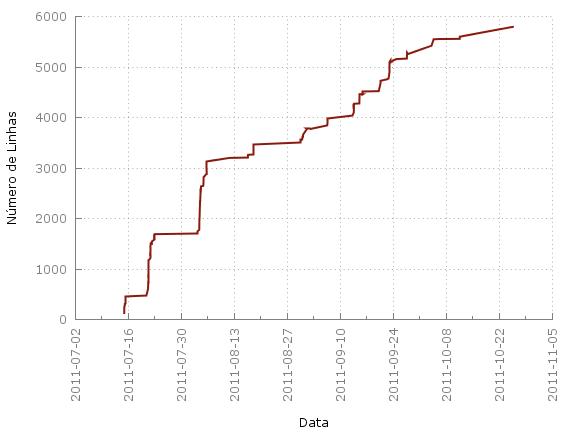
\includegraphics[width=0.8\textwidth]{./imgs/lines_of_code.png}
}

\frame
{
\frametitle{Metodologia Empregada}
Evolução do número de linhas de código do projeto por programador ao longo do processo de desenvolvimento.
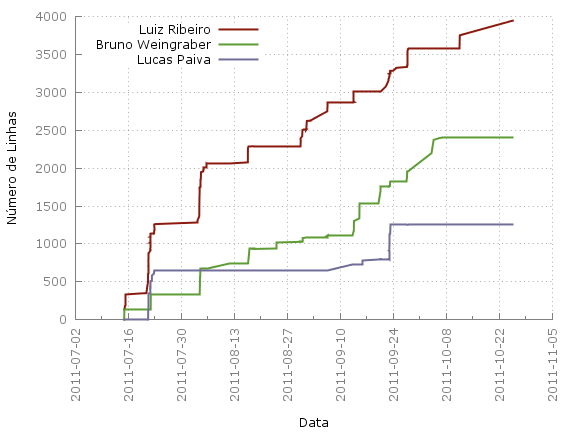
\includegraphics[width=0.8\textwidth]{./imgs/lines_of_code_by_author.png}
}

\frame
{
\frametitle{Metodologia Empregada}
Número de \emph{commits} por dia de semana.
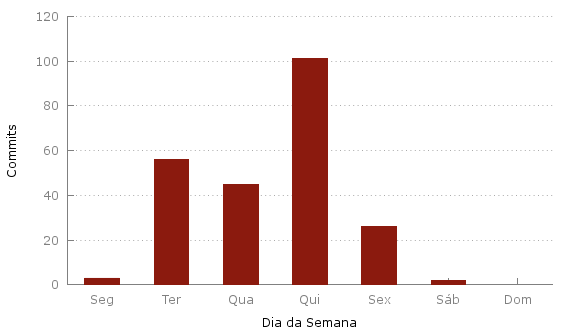
\includegraphics[width=0.8\textwidth]{./imgs/day_of_week.png}
}

\frame
{
\frametitle{Metodologia Empregada}
Número de \emph{commits} por horário.
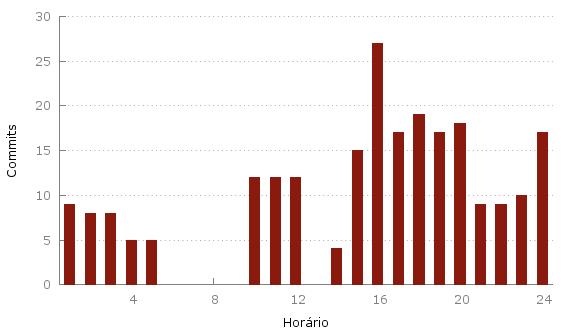
\includegraphics[width=0.8\textwidth]{./imgs/hour_of_day.png}
}

\subsection{Performance do Sistema}
\frame
{
\frametitle{Teste de \emph{stress}}
Execução de uma série de consultas simultâneas para avaliação do tempo de resposta do sistema.
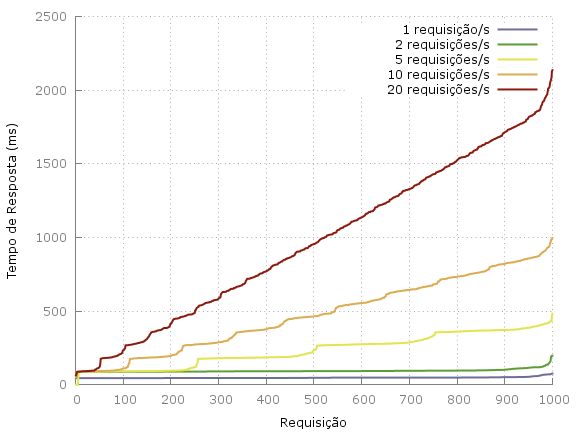
\includegraphics[width=0.8\textwidth]{./imgs/out.png}
}